\documentclass[twocolumn,pra,showpacs,superscriptaddress,longbibliography]{revtex4-1}   % use preprint or twocolumn
\usepackage{graphicx}
\usepackage{amsmath}
\usepackage{amssymb}
\usepackage{epstopdf}
\usepackage{dcolumn}% Align table columns on decimal point
\usepackage{bm}% bold math
\usepackage{verbatim}
\usepackage{amsfonts}
\usepackage{cancel}
\usepackage[utf8]{inputenc}
\usepackage{graphicx}
\usepackage{setspace}
\usepackage{tabularx}
\usepackage[export]{adjustbox}



\DeclareGraphicsRule{.tif}{png}{.png}{`convert #1 `dirname #1`/`basename #1 .tif`.png}


\newcommand{\sspace}{$\enspace$}
\newcommand{\ssspace}{$\quad$}
\newcommand{\proofend}{\mbox{ }\hfill$\Box$\\}
\newcommand{\deriv}[2]{\frac{\mathrm{d} #1}{\mathrm{d} #2}}
\newcommand{\parderiv}[2]{\frac{\partial #1}{\partial #2}}
\newcommand{\ee}[1]{\cdot 10^{ #1}}
\newcommand{\bra}[1]{\left\langle #1 \right|}
\newcommand{\ket}[1]{\left| #1 \right\rangle}
\newcommand{\braopket}[3]{\left.\left\langle #1 \right|\right|#2\left|\left| #3 \right\rangle\right.}
\newcommand{\dbbraopket}[3]{\left.\left\langle#1\right.\right.\|#2\|\left.\left.#3\right\rangle\right.}
\newcommand{\braket}[2]{\left\langle #1 \right|\left. #2 \right\rangle}
\newcommand{\trace}[1]{\mathrm{Tr}\left(#1\right)}
\newcommand{\abs}[1]{\left|#1\right|}
\newcommand{\avg}[1]{\left\langle #1 \right\rangle}
\newcommand{\figref}[1]{Fig.~\ref{#1}}
\newcommand{\eqnref}[1]{Eqn.~\eqref{#1}}


\newcommand{\AAA}{\mathrm{\AA}}

\newcommand{\abinit}{\textit{ab initio}}
\newcommand{\abinitspace}{\textit{ab initio} }




\begin{document}

\title{Notes on calculating atom interferometer gyroscope sensitivity}
\maketitle


\subsection{Theory}

The goal of this project is to allow us to explore how the sensitivity of a Mach-Zehnder atom interferometer gyroscope is determined by:
\begin{itemize}
	\item choice of atom (and its associated van der Waals $C_3$ coefficient)
	\item atom velocity $v$
	\item grating period $d_g$
	\item grating open fractions $f = w/d_g$, where $w$ is the width of the gaps between adjacent grating bars
	\item grating longitudinal thickness $l$.
	\item longitudinal distance between successive gratings $L$
\end{itemize}
Choosing the grating thickness $l$ and grating-to-grating distance $L$ is likely fairly simple: we always want smaller $l$ and larger $L$, but $l$ will probably be determined by the grating fabrication process and $L$ is limited by the maximum size of the apparatus. The grating period $d_g$ and open fraction $w/d_g$ can be optimized for a choice of atom and atom velocity $v$. Therefore, we want to be able to plot the sensitivity of a Mach-Zehnder atom interferometer gyroscope as a function of $v$ for different atoms.

The sensitivity $S$ of a gyroscope is described as 
\begin{align}
	S = \delta\Omega \sqrt{t}
	\label{sensitivityGeneral}
\end{align}
where $\delta\Omega$ is the uncertainty in a typical measurement of rotation rate $\Omega$ and $t$ is the amount of data acquisition time required to make that measurement. 
Smaller values of $S$ are preferable.
Values of $S$ are usually expressed in rad/s/$\sqrt{\mathrm{Hz}}$. 
$S$ also is a measure of the uncertainty in the gyroscope's angular orientation as a function of operating time and is therefore sometimes expressed in $^{\circ}/\sqrt{h}$ (i.e. the uncertainty in the gyroscope's angular orientation is $S\sqrt{T}$, where $T$ is the operating time since last calibration).

This sensitivity $S$ can be written in terms of the items listed previously.
For an atom interferometer gyroscope, the phase $\phi$ can be written as
\begin{align}
	\phi = \frac{4\pi\vec{\Omega}\cdot\vec{A}}{\lambda_{dB} v} - \phi_0
\end{align}
where $\phi_0$ is an arbitrary refrence phase, $\lambda_{dB}$ is the atoms' de Broglie wavelength, and $\vec{\Omega}\cdot\vec{A}$ is the projection of the gyroscope's rotation rate vector $\vec{\Omega}$ onto the plane of the interferometer with enclosed area $A$. If we let $\Omega$ be the component of $\vec{\Omega}$ normal to $\vec{A}$ and represent $\lambda_{dB}$ as $h/mv$, we can rewrite the above equation as
\begin{align}
	\delta\phi = \frac{4\pi m A}{h}\delta\Omega
\end{align}
and solve it for $\delta\Omega$ to get
\begin{align}
	\delta\Omega = \frac{h}{4\pi m A}\delta\phi
	\label{deltaOmega}
\end{align}

According to \cite{Lenef1997}, the uncertainty $\delta\phi$ on a single measurement of the phase of an atom interferometer is defined by
\begin{align}
	\delta\phi^2 = \frac{1}{|C|^2N}
	\label{phaseSDev}
\end{align}
where $N$ is the number of atoms detected.
Substituting Eq. \ref{phaseSDev} into Eq. \ref{deltaOmega} and the result into Eq. \ref{sensitivityGeneral}, we get 
\begin{align}
	S = \frac{h}{4\pi m A} \sqrt{\frac{t}{|C|^2N}}
	\label{sensitivity2}
\end{align}
If we take $t$ to be the unit time, we see $N/t$ is the average atom beam intensity (i.e. flux) $\avg{I}$.

The interferometer's enclosed area $A$ can be written as
\begin{align}
	A = L^2\tan{\theta_d} = L^2\tan\left(\arcsin\left(\frac{h}{mvd_g}\right)\right) \approx \frac{L^2h}{mvd_g}
\end{align}
Substituting into Eq. \ref{sensitivity2}, we get
\begin{align}
	S = \frac{vd_g}{4\pi L^2} \frac{1}{ \sqrt{|C|^2\avg{I}}}
	\label{sensitivity3}
\end{align}


\cite{Cronin2005} describes in detail how to calculate $|C|^2\avg{I}$ from the nanograting open fraction, thickness, and period as well as atom velocity and atom-grating $C_3$ coefficient. This calculation can be done with and without considering van der Waals interactions between the atoms and the grating bars. 
Kapitza-Dirac gratings can be represented as gratings for which $C_3 = 0$ and the open fraction $f = 1/2$.

Note that the $\left(e_n^{Gi}\right)^2$ terms in Eq. 14 in \cite{Cronin2005} should actually be written as $\left|e_n^{Gi}\right|^2$.

van der Waals $C_3$ coefficients for alkali metals interacting with various media (including silicon nitride) are listed in atomic units in \cite{Arora2014}. To convert the $C_3$ coefficients in atomic units to SI units (for the sake of the numerical calculations), multiply by 1 Hartree times the Bohr radius cubed. Useful $C_3$ coefficients are listed in atomic units in Table \ref{tableC3}.

\begingroup
\begin{table}
\caption{\label{tableC3} van der Waals $C_3$ coefficients in atomic units for various combinations of atoms and dielectric media \cite{Arora2014}.}
\begin{center}
\begin{tabular}{l|ll}
\hline\hline
& SiN$_x$ & SiO$_2$ \\
\hline
Li & 0.715 & 0.484 \\
Na & 0.794 & 0.5424 \\
K &  1.212 & 0.839 \\
Rb & 1.369 & 0.956 \\
\hline\hline
\end{tabular}
\end{center}
\end{table}
\endgroup


\subsection{Results}

\begin{figure}
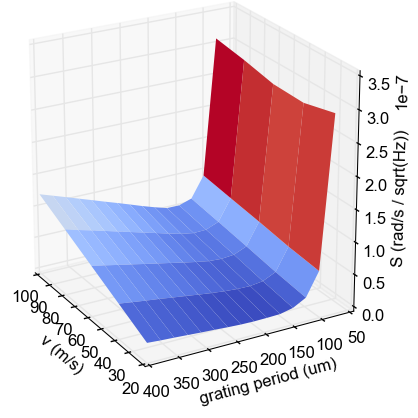
\includegraphics[width=\linewidth,keepaspectratio]{../plots/Sf1f2_vs_dv_Rb_L10cm_cropped.png}
\caption{\label{S_vs_dv} Sensitivity of a Rb atom interferometer gyroscope vs velocity and SiN$_x$ grating period assuming $L=10$ cm. For each point on this plot, the optimal open fractions were calculated. The optimal open fractions were restricted to a grating-period-dependent maximum, which corresponds to a minimum grating bar width of 40 nm. Lower $S$ is preferable.}
\end{figure}

\begin{figure}
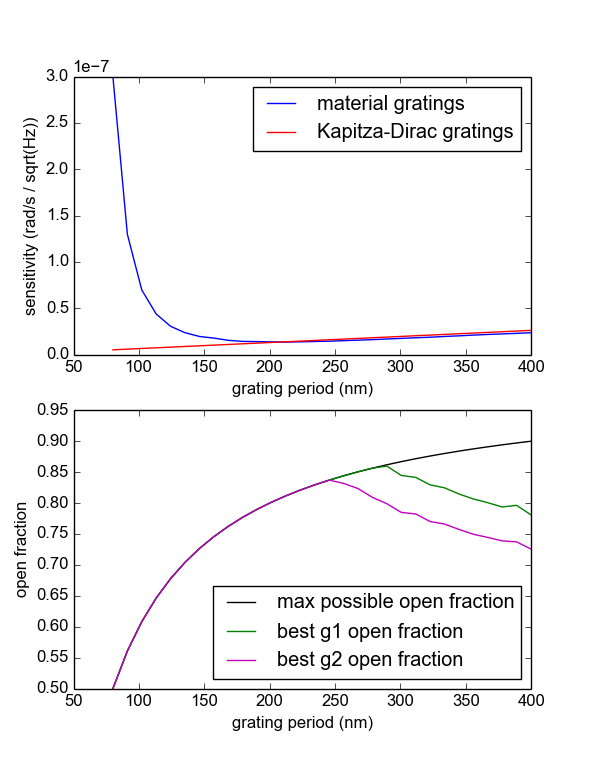
\includegraphics[width=\linewidth,keepaspectratio]{../plots/Sf1f2_vs_d_Rb_L10cm.png}
\caption{\label{S_vs_d} Sensitivity of a Rb atom interferometer gyroscope vs SiN$_x$ grating period for $v=20$ m/s, $L=10$ cm and the optimal open fractions that correspond to that sensitivity. The maximum open fractions were calculated assuming a minimum grating bar width of 40 nm. Lower $S$ is preferable.}
\end{figure}


Fig \ref{S_vs_dv} shows the sensitivity of an atom interferometer gyroscope with material gratings as a function of $v$ and $d_g$. For this calculation, it was assumed that $L = 10$ cm and the $C_3$ coefficient was that of Rb interacting with SiN$_x$. For each $(v,d)$ coordinate on the plot, the sensitivity $S$ was optimized with respect to the grating 1 and grating 2 open fractions $f_1$ and $f_2$. For this optimization, $f_1$ and $f_2$ were allowed to vary between 0 and $1 - w_{min}/d$, where $w_{min}$ is the minimum width of a single grating bar that is allowed by the nanograting fabrication process and that will not cause the grating to fall apart. For these calculations, $w_{min} = 40$ nm, although that number is essentially just a guess.
Fig \ref{S_vs_dv} indicates that sensitivity $S$ always improves as $v$ decreases, which is convenient for the low speeds associated with launching atoms out of a 2D MOT.

Fig \ref{S_vs_d} shows a slice of Fig \ref{S_vs_dv} at $v=20$ m/s. We can see that $S$ is optimized when $d_g=200$ nm. Fig \ref{S_vs_d} also shows the optimal open fractions, along with the maximum open fractions, as a function of $d_g$.  At $d_g=200$ nm, the optimal open fractions are equal to the maximum open fractions, which impies that $S$ could be further improved by reducing $w_{min}$. 

From Fig \ref{S_vs_d}, we can also see that material gratings are preferable to Kapitza-Dirac gratings in terms of both SWP and sensitivity. While $S$ appears to decrease monotonically as $d_g$ decreases for K-D gratings, obtaining a CW laser, and the optics for that laser, much below 350 nm is essentially impossible. As a side note, the reason the material gratings sensitivity is slightly lower than the K-D sensitivity for $d_g > 200$ nm is because K-D gratings are restricted to 50\% open fractions, whereas material gratings can have more optimal open fractions.


\begin{figure}
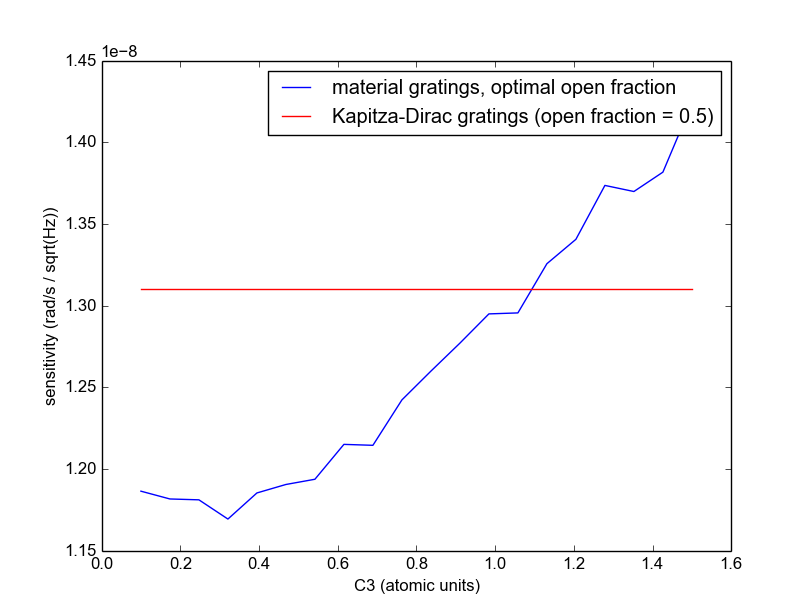
\includegraphics[width=\linewidth,keepaspectratio]{../plots/S_vs_C3_d200nm_v20_L10cm.png}
\caption{\label{S_vs_C3} Sensitivity of a Rb atom interferometer gyroscope vs the van der Waals $C_3$ coefficient for interaction between the atoms and the gratings at $d_g=200$ nm, $v=20$ m/s, $L=10$ cm and optimal open fractions.}
\end{figure}

Fig \ref{S_vs_C3} shows how sensitivity depends on the van der Waals $C_3$ coefficient associated with interaction between the atoms and the grating bars. For this calculation, it was assumed that $v=20$ m/s, $d_g=200$ nm, and $L = 10$. This calculation suggests that using K or Na rather than Rb is probably not worth the effort of developing a new K source, which may involve temperatures that are unreasonably high for this application. 

Note that $L$ only appears outside the expression for $\sqrt{|C|^2\avg{I}}$ in Eq. \ref{sensitivity3}. This means that the length of the interferometer has no bearing on the optimal $v$, $d_g$, $C_3$, or open fractions. Therefore, we simply want $L$ to be as long as possible given the size constraints of the apparatus. If the apparatus must exist in a box, then we could consider orienting the interferometer to stretch between opposite corners. 

For these calculations, I used $l = 150$ nm because that is the longitudinal thickness of the grating bars in our atom interferometer at University of Arizona.

Based on the calculations presented here, I propose to build a nanograting atom interferometer gyroscope with the following specifications:
\begin{itemize}
	\item atom: Rb (because we already have Rb source and optics)
	\item $v$: 20 m/s (typical 2D MOT output, lower is better)
	\item $d_g$: 200 nm
	\item open fractions $f_{g1} = 0.8$, $f_{g2} = 0.8$, $f_{g3} = 0.37$ 
	\item $l=150$ nm (estimated lower limit)
	\item $L=10$ nm (estimated upper limit)
\end{itemize}
An interferometer with these specifications would have an optimal sensitivity of $S = 2.0\cdot10^{-8}$ rad/s/$\sqrt{\mathrm{Hz}}$, which corresponds to an ARW of $6.9\cdot10^{-5}$ $^{\circ}/\sqrt{h}$. While the state-of-the-art, table-top, atom interferometer gyroscopes have a sensitivity that is an order of magnitude better \cite{Durfee2006}, a portable, low-SWP system such as the one described here represents a significant advancement for the field.



\bibliography{library}

\end{document}  